\documentclass{oci}
\usepackage[utf8]{inputenc}
\usepackage{lipsum}
% \usepackage[spanish]{babel}

\problem{C}
\phase{Clasificatoria Regional}
\title{Colección de láminas}


\begin{document}
\begin{problemDescription}
Jorge es un niño que tiene una única pasión en la vida: coleccionar láminas para completar sus álbumes favoritos.
% Cada álbum está compuesto por cierta cantidad de láminas y para completarlo es necesario conseguirlas todas.
El último álbum que Jorge logró completar fue el de los Lokómones.
En la imagen de abajo se muestran algunas de las láminas del álbum.

\begin{center}
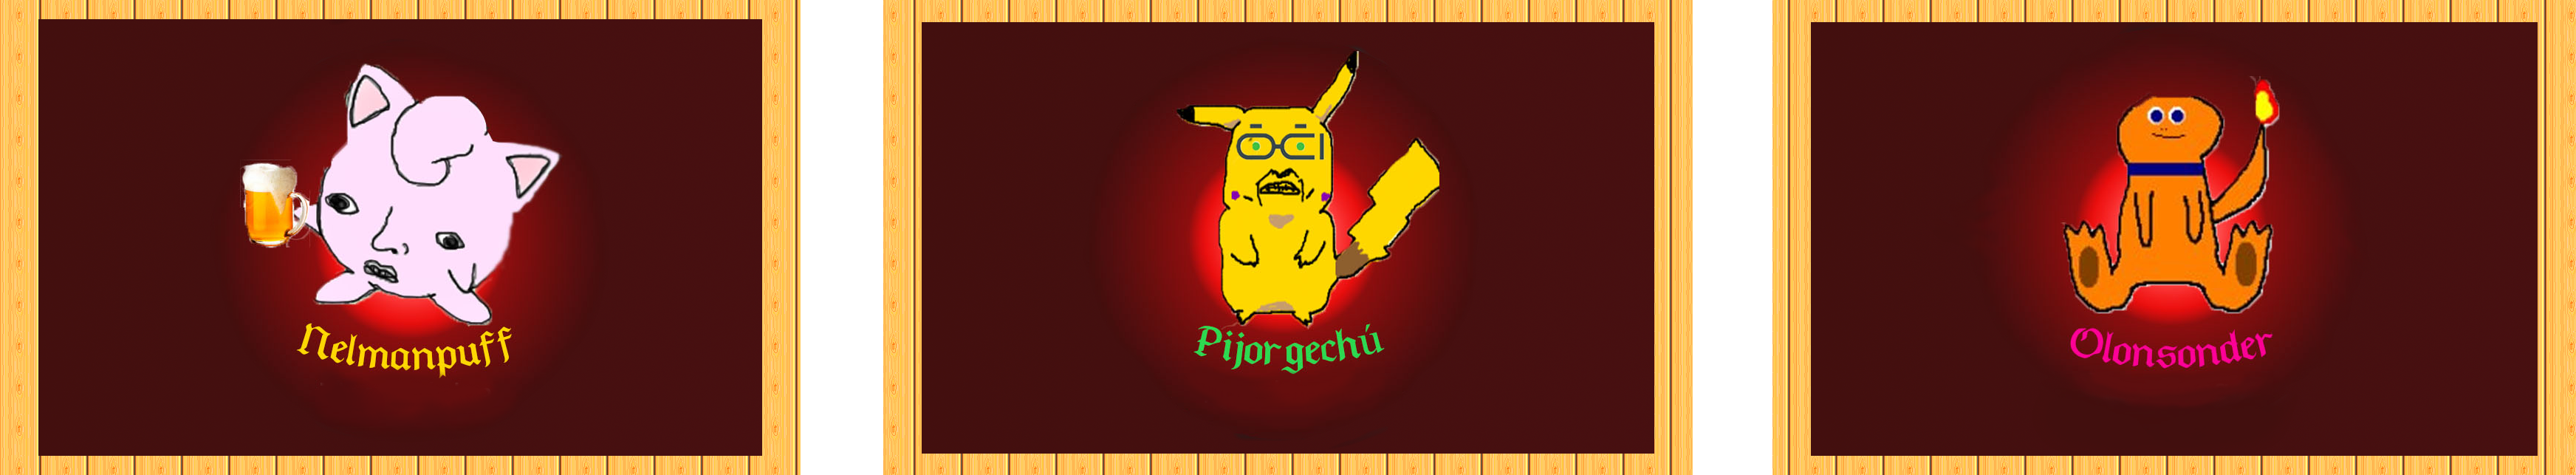
\includegraphics[scale=0.5]{locomons-laminas.png}
\end{center}

Para completar los álbumes Jorge debe comprar sobres con láminas.
Cada uno de los sobres contiene 5 láminas, pero Jorge no sabe qué láminas le saldrán antes de comprarlos.
Es por esto que siempre debe comprar muchos sobres extras, pues es muy probable que al comprarlos le salgan láminas que ya tenía.
% Esto es un problema pues los sobres son bastante caros y las láminas repetidas no le sirven para nada, ni siquiera para intercambiarlas con otras personas, pues Jorge no tiene amigos.

Luego de completar su último álbum, el de los Lokómones, Jorge se enteró que también era posible comprar láminas sueltas escogiendo las que quisiera.
Si Jorge se hubiese enterado antes de esto no habría acumulado tantas láminas repetidas, pues simplemente podría haber comprado las láminas que le faltaban.

Jorge además se pregunta si comprando láminas sueltas podría haber gastado menos dinero.
% No es tan sencillo darse cuenta de esto, pues algunas láminas, al ser más ``raras'', son más caras que otras al comprarlas sueltas.
Él cree que hubiese sido conveniente comprar sobres hasta cierto punto y luego de eso comprar sueltas todas las láminas que no alcanzó a recolectar con los sobres.
% Además de coleccionar láminas Jorge no tiene muchas otras habilidades y le está costando encontrar cuál hubiera sido el momento óptimo donde dejar de comprar sobres.
Por suerte Jorge es un niño muy ordenado y anotó las láminas que le salieron en cada uno de los sobres que compró. ?`Podrías ayudarlo?

El álbum consiste en $N$ láminas y por simplicidad nos referiremos a ellas con números del 1 al $N$.
Cada sobre tiene un precio $P$ y contiene 5 láminas.
% Además sabes el precio asociado a la compra de cada lámina suelta y las láminas que salieron en cada sobre que compró Jorge.
Además sabes el precio asociado a la compra de cada lámina suelta.
Tu tarea es encontrar la mínima cantidad de dinero que Jorge podría haber gastado para completar todo el álbum si hubiese dejado de comprar sobres en algún punto y luego hubiese comprado láminas sueltas.
\end{problemDescription}

\begin{inputDescription}
La primera línea de la entrada contiene tres enteros positivos separados por un espacio.
Estos corresponden respectivamente a la cantidad de láminas del álbum ($N$), la cantidad de sobres comprados por Jorge ($S$) y el precio de cada sobre ($P$).

La segunda línea contiene $N$ enteros positivos separados por espacios correspondientes a los precios de cada lámina.
El primer entero al precio de la lámina 1, el segundo al precio de la lámina 2, etc.
El precio de cada lámina será mayor o igual que 1 y menor o igual que 5000.

Las siguientes $S$ líneas contienen la descripción de cada sobre que compró Jorge.
Cada una de estas líneas contiene 5 enteros entre 1 y $N$ describiendo las láminas que salieron en el sobre.
Debes asumir que considerando todos los sobres es posible juntar las $N$ láminas. 
Además Jorge no compró sobres extras, es decir, en el último sobre obtuvo las últimas láminas que le faltaban.
\end{inputDescription}

\begin{outputDescription}
Debes imprimir un solo entero correspondiente a la mínima cantidad de dinero que podría haber gastado Jorge si solo hubiese comprado sobres hasta cierto punto y luego hubiese comprado el resto de las láminas sueltas.
\end{outputDescription}

\begin{scoreDescription}
  \score{30} Se probarán varios casos donde
 $0 < N \leq 10,\ 0 < S \leq 2,\ 0 < P \leq 100$ y no hay restricciones adicionales.
  \score{25} Se probarán varios casos donde
 $10 < N \leq 500,\ 2 < S \leq 100,\ 0<P\leq 5 $ y nunca salen láminas repetidas.
 %  \score{25} Se probarán varios casos donde
 % $0<P\leq 1000,\ 100 < S \leq 1000,\ 500 < N \leq 5000$ y todas las láminas sueltas tienen el mismo precio.
  \score{45} Se probarán varios casos donde
 $500<N\leq 5000,\ 100 < S \leq 1000,\ 0<P\leq 1000$ y no hay restricciones adicionales.
\end{scoreDescription}

\begin{sampleDescription}
\sampleIO{sample1}
\sampleIO{sample2}

En el primer ejemplo el álbum está compuesto por 7 láminas.
Jorge compró 4 sobres y cada uno costó 5 unidades.
En este caso a Jorge le hubiese convenido comprar solo hasta el segundo sobre.
De esta forma Jorge hubiese conseguido las láminas 3, 4, 5, 6 y 7 gastando 10 unidades en sobres.
Luego podría haber comprado las láminas 1 y 2 por 5 y 4 unidades respectivamente para un total de 19 unidades sumando a lo que había gastado en sobres.
Notar que Jorge podría haber gastado la misma cantidad de dinero si hubiese comprado hasta el tercer sobre y luego la lámina 2 suelta.

En el segundo ejemplo comprar láminas sueltas no hubiese ayudado a Jorge y lo óptimo hubiese sido comprar todos los sobres por 5 unidades cada uno para un total de 20 unidades.

\end{sampleDescription}

\end{document}
